
%(BEGIN_QUESTION)
% Copyright 2011, Tony R. Kuphaldt, released under the Creative Commons Attribution License (v 1.0)
% This means you may do almost anything with this work of mine, so long as you give me proper credit

In this biogas generation system, cow manure is used as a feedstock to produce methane gas (CH$_{4}$), which is then used to fuel an engine to turn a generator and make electricity.  The waste heat from the engine is used to maintain the cascaded digesters (``reactors'' R-101 and R-102) at optimal temperatures for anaerobic bacteria to digest the manure and produce biogas (approximately 105 $^{o}$F):

$$\includegraphics[width=15.5cm]{i00069x01.eps}$$

\begin{itemize}
\item{} What kind of control valves are TV-41 and TV-48?
\vskip 10pt
\item{} Assuming LT-55 is a direct-acting level transmitter and LIC-55 is a reverse-acting level controller, determine the necessary split-range calibrations of LV-55a and LV-55b.
\vskip 10pt
\item{} What would the consequence(s) be if TT-43 failed with a high signal?
\end{itemize}

\vfil 

\underbar{file i00069}
\eject
%(END_QUESTION)





%(BEGIN_ANSWER)

This is a graded question -- no answers or hints given!

%(END_ANSWER)





%(BEGIN_NOTES)

TV-41 and TV-48 are both {\it 3-way} or {\it diverter} valves, sometimes called {\it mixing} valves if used to bring two streams together.  In this case, they both serve to divert engine coolant flow around heat exchangers to control temperature.

\vskip 10pt

Control valves LV-55a and LV-55b must be {\it complementarily} split-ranged, because we need the two to act in harmony to divert flow out of reactor R-101 to either R-102 or back through the heat exchanger and into R-101 again.  At no time do we ever wish to close off both of these valves, because that would cause the pump discharging material from R-101 to become ``dead-headed'' (i.e. pumping into a blocked line).  Given that LIC-55 is reverse-acting, a high liquid level inside of R-101 will produce a low controller output, which is the condition where we desire LV-55a to be open further than LV-55b.  Thus, LV-55a needs to be wide-open at 4 mA (signal-to-close, fail-open) and LV-55b needs to be wide open at 20 mA (signal-to-open, fail-closed):

$$\includegraphics[width=15.5cm]{i00069x02.eps}$$

\begin{itemize}
\item{} LV-55a (flow out to R-102): 4 mA = wide open ; 20 mA = shut
\item{} LV-55b (R-101 recirculation): 4 mA = shut ; 20 mA = wide open
\end{itemize}

\vskip 10pt

If TT-43 failed high, TIC-43 would ``think'' the engine was too hot, and run the fin-fan speed at maximum all the time.  The result of this would be the engine running too cool, and possibly the digesters (R-101 and R-102) running too cool as well, causing biogas production to decrease.

%INDEX% Basics, control: direct versus reverse controller action
%INDEX% Final Control Elements, valve: P&ID symbols
%INDEX% Process: anaerobic digester (manure)

%(END_NOTES)


